\documentclass[t,darkblue]{beamer}
\usepackage[portuguese]{babel}
\usepackage[utf8]{inputenc}
\usepackage{times}
\usepackage[T1]{fontenc}
\usepackage{hyperref}
\usepackage[alf]{abntex2cite}
\usepackage{tikz}
\usepackage{listings}
\usepackage{xcolor}
\usepackage[export]{adjustbox}
\usepackage{lipsum}
\usepackage{caption}			% Pacote para retirar o prefixo "Figura"
\captionsetup[figure]{labelformat=empty}% redefines the caption setup of the figures environment in the beamer class.
\usepackage{parskip}
\setlength{\parskip}{\baselineskip} 

\renewcommand{\raggedright}{\leftskip=0pt \rightskip=0pt plus 0cm}
\newcommand\fontvi{\fontsize{9}{9}\selectfont}

% Definição de estilo

\usetheme{Madrid} 
%\setbeamertemplate{background}{\tikz[overlay,remember picture]\node[opacity=0.4]at (current page.center){\includegraphics[width=2cm]{Imagens/Logomarca}};} % Marca d'água por trás do texto

% Definição de fonte
\usefonttheme[onlylarge]{structurebold}
\setbeamerfont*{frametitle}{size=\normalsize,series=\bfseries}

% Definição de cores
\definecolor{icmcAzulLogo}{RGB}{121,178,242}
\definecolor{icmcAzulSite}{RGB}{66,135,214}
\definecolor{icmcAzulBorda}{RGB}{66,135,214}

% Range de cores do template
\setbeamercolor{structure}{fg=icmcAzulBorda!90!icmcAzulSite}

% Declaração alternativa da palheta de cores do modelo
%\mode<presentation>
%{
%	\usetheme{Madrid}
%	\setbeamercolor*{palette primary}{use=structure,fg=white,bg=icmcAzulSite}
%	\setbeamercolor*{palette secondary}{use=structure,fg=white,bg=icmcAzulLogo}
%	\setbeamercolor*{palette tertiary}{use=structure,fg=white,bg=icmcAzulBorda}
%}

\begin{document}
	\author[Projeto 1]{Projeto1: Plano de Ação a Combate a Incêndio}
	\title[Projeto 1: Fogo e GIS]{Como dominar o mundo com geoprocessamento}
	\subtitle{Aulas 7 - 10}
	\titlegraphic{\vspace{-1cm}
\includegraphics[width=2.0cm]{./image/vale}\hspace*{6.75cm}~%
		
\includegraphics[width=1.5cm]{./image/qgis}\\
		
\includegraphics[width=2.5cm]{./image/tetra}}
	\institute[]{Alexandre Assunção}
	\date{26 de agosto de 2025}
	%\subject{}
	%\setbeamercovered{transparent}
	\setbeamertemplate{navigation symbols}{}
	\begin{frame}[plain]
	\maketitle
	\end{frame}

% Conteúdo
\begin{frame}
\frametitle{Sumário do Projeto}
\large
\begin{itemize}
	\item Introdução;
	\item Consulta de dados em repositórios;
	\item Familiarização com os dados;
	\item Análises espaciais;
	\item ;
\end{itemize}
\end{frame}


\begin{frame}
	\frametitle{Introdução}
	\begin{figure}[H]
		\centering
		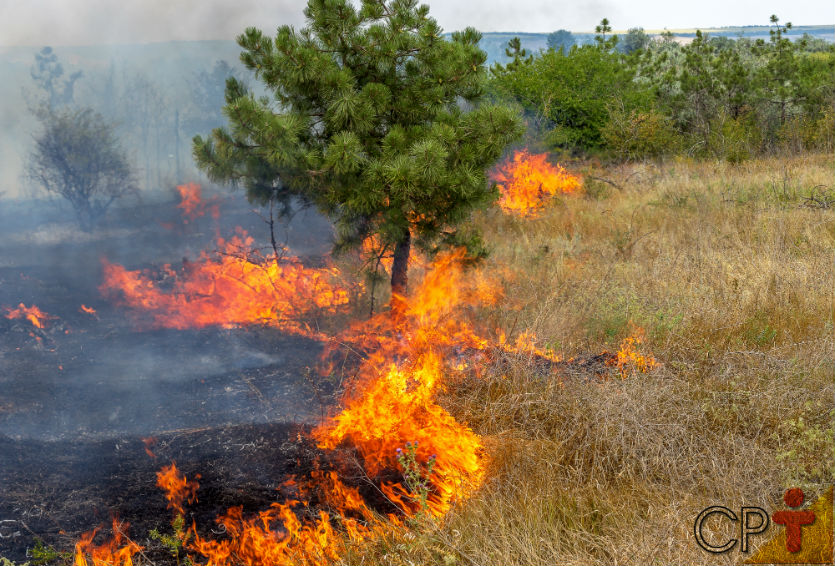
\includegraphics[width=\textwidth]{./image/incendio_florestal.jpg}
	\end{figure}
\end{frame}

\begin{frame}
	\frametitle{Introdução}
	\begin{figure}[H]
		\centering
		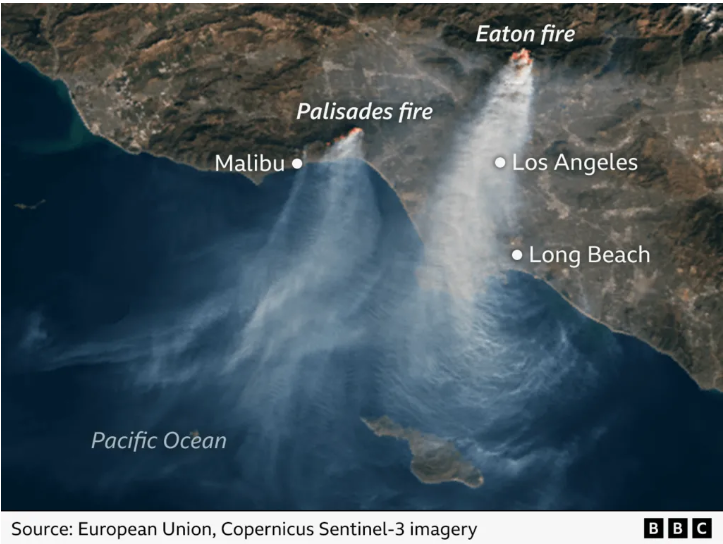
\includegraphics[width=\textwidth]{./image/bbc_image.png}
	\end{figure}
\end{frame}

\begin{frame}
	\frametitle{Introdução}
	\begin{figure}[H]
		\centering
		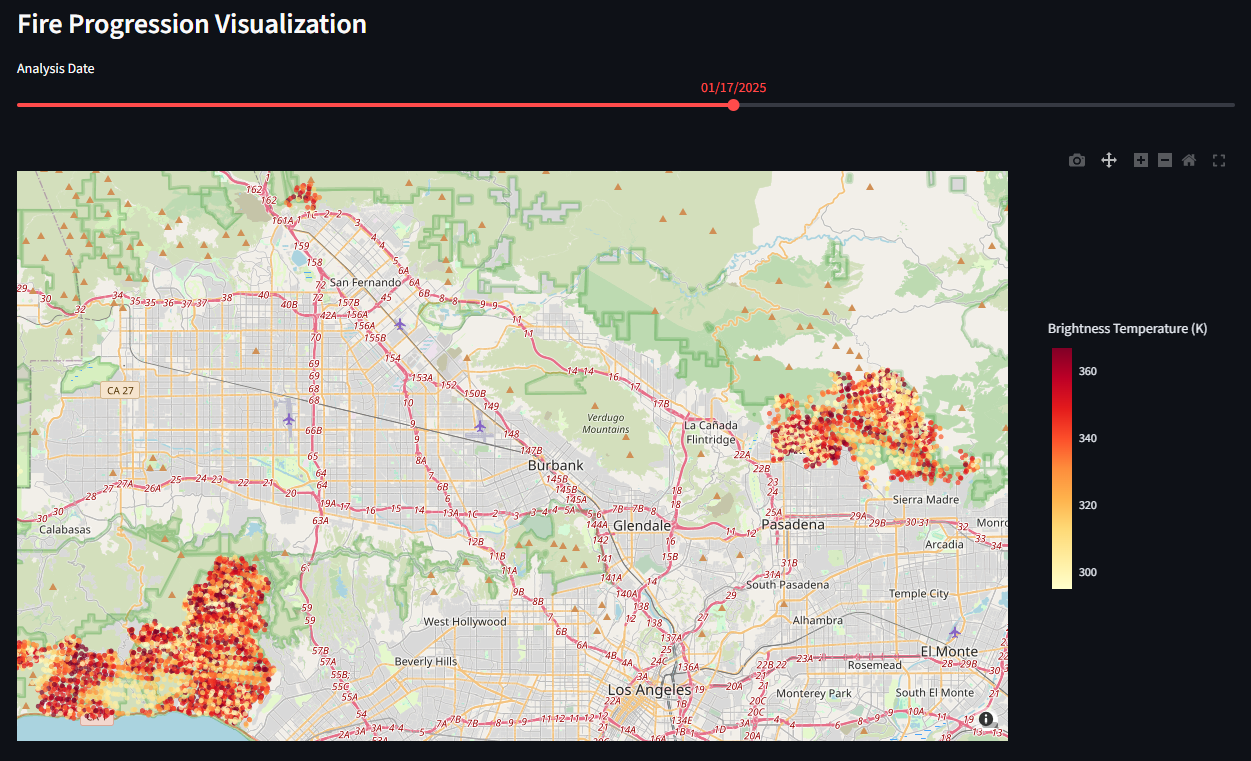
\includegraphics[width=0.8\textwidth]{./image/app_la.png}
	\end{figure}
	\href{https://localsolve-la-wildfires.streamlit.app/}{Link App}
\end{frame}


\begin{frame}
	\frametitle{Introdução}
	\begin{figure}[H]
		\centering
		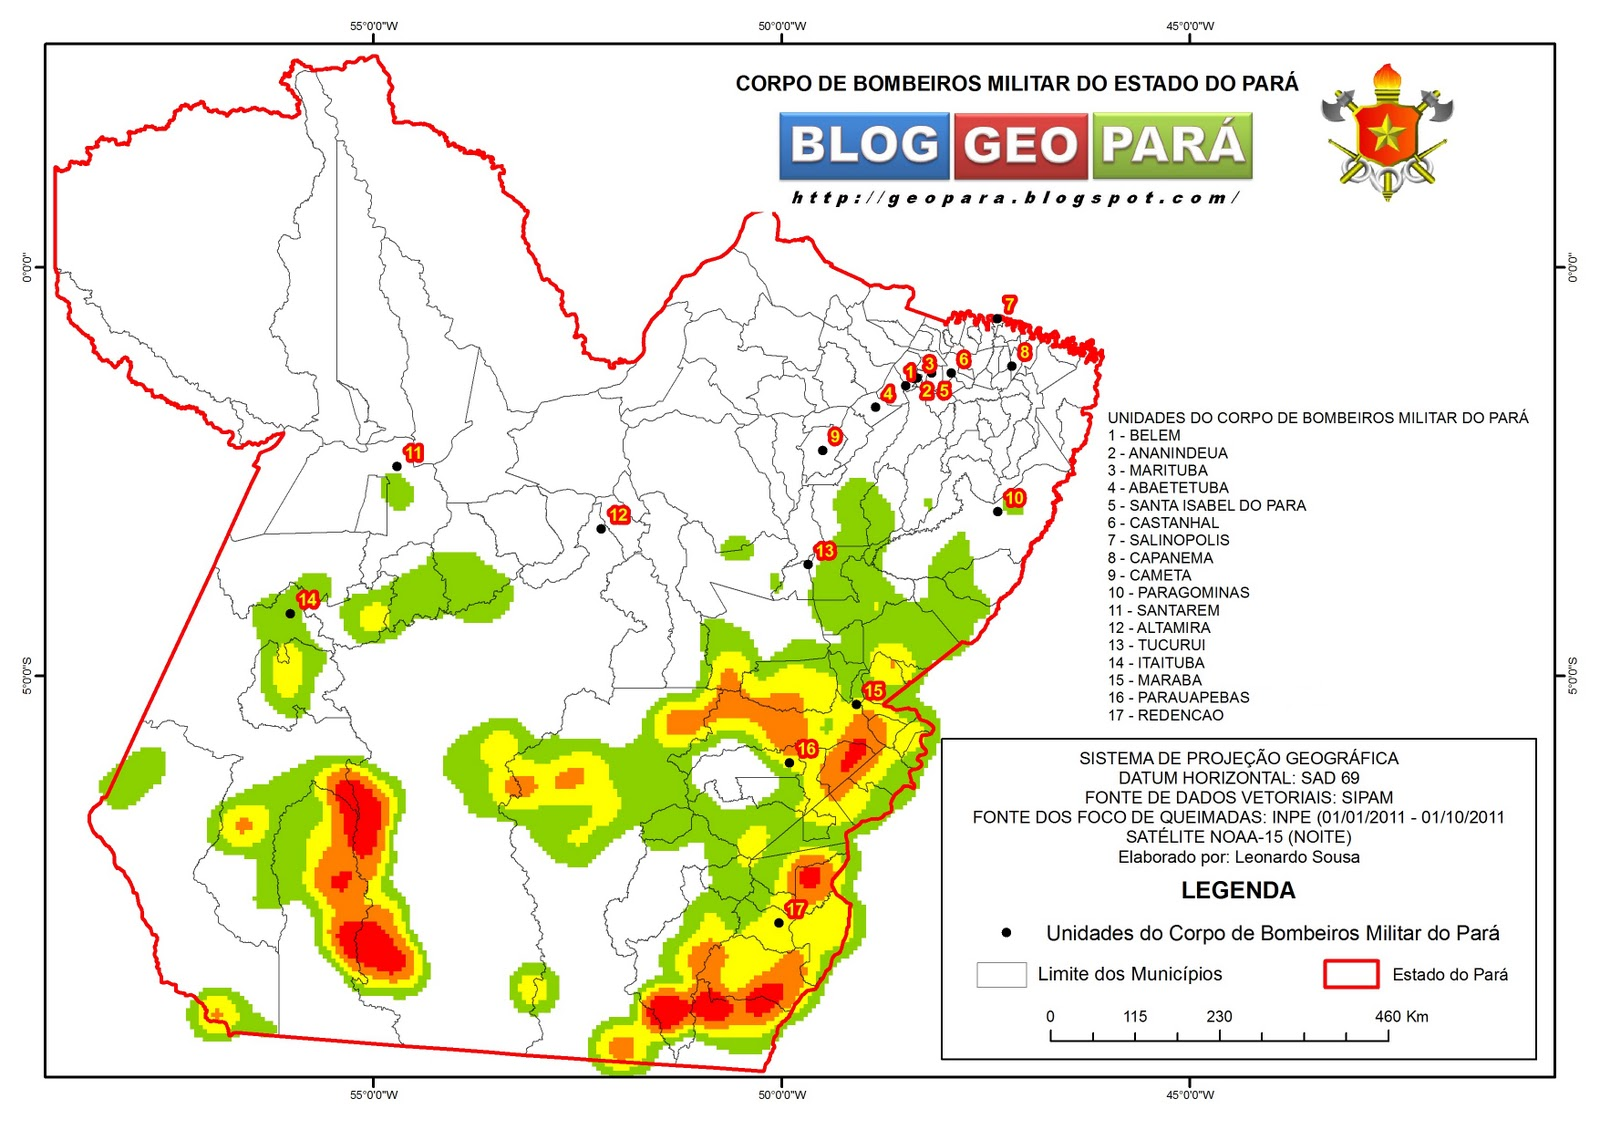
\includegraphics[width=\textwidth]{./image/mapa_incendio_para.jpg}
	\end{figure}
\end{frame}

\begin{frame}
	\frametitle{Introdução}
	\begin{figure}[H]
		\centering
		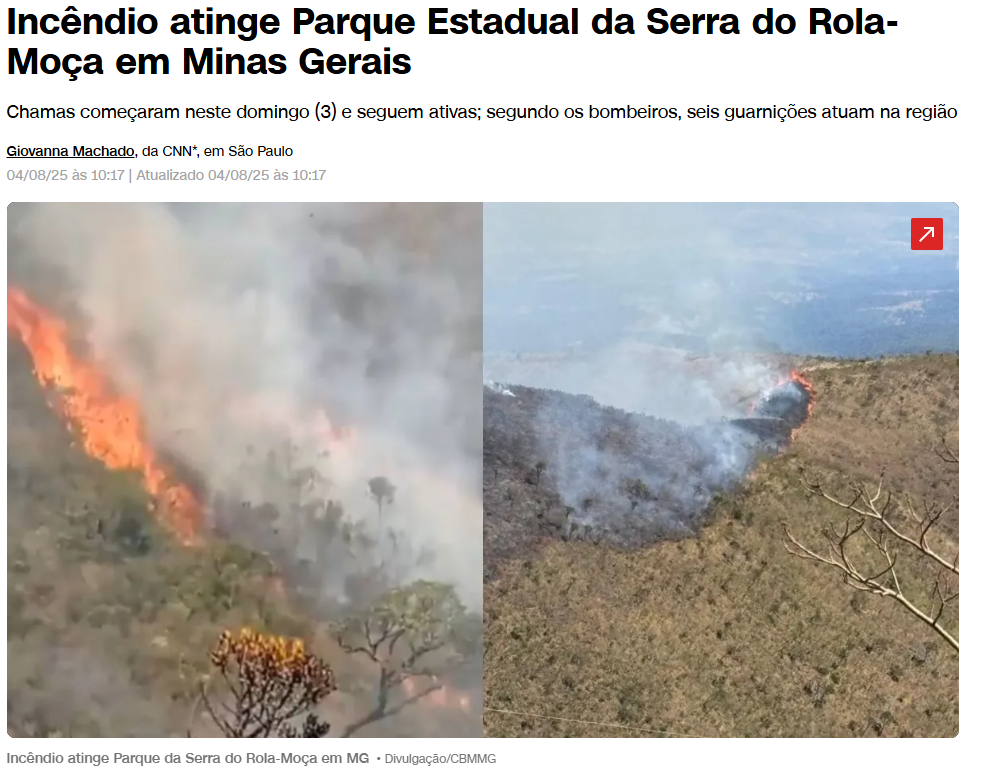
\includegraphics[width=\textwidth]{./image/incendio_rola_moca.png}
	\end{figure}
\end{frame}


\begin{frame}
	\frametitle{Introdução}
	\begin{figure}[H]
		\centering
		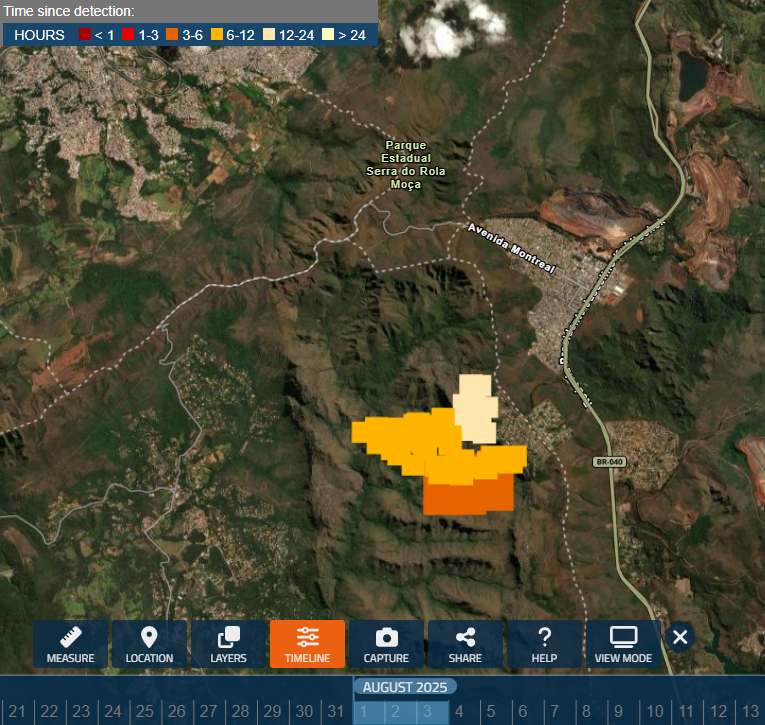
\includegraphics[width=\textwidth]{./image/nasa_incendio_rola_moca.png}
	\end{figure}
\end{frame}


\begin{frame}
	\frametitle{Introdução}
	\begin{figure}[H]
		\centering
		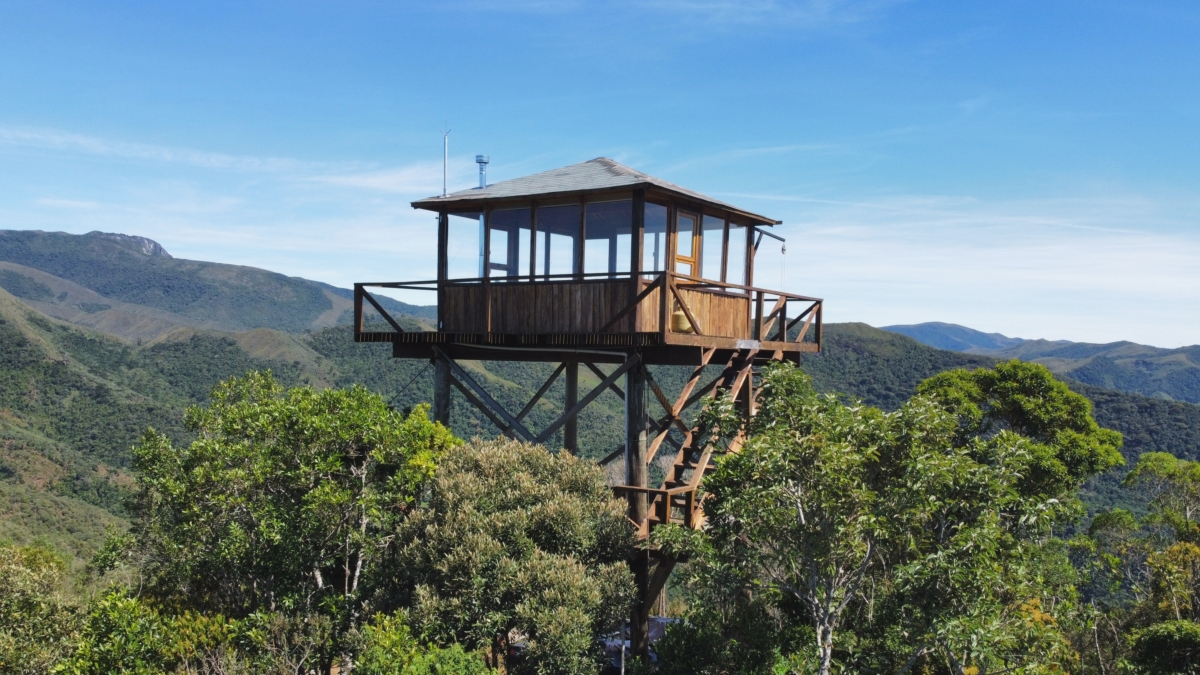
\includegraphics[width=\textwidth]{./image/torre_observacao}
	\end{figure}
\end{frame}


\begin{frame}
	\frametitle{Introdução}
	\begin{figure}[H]
		\centering
		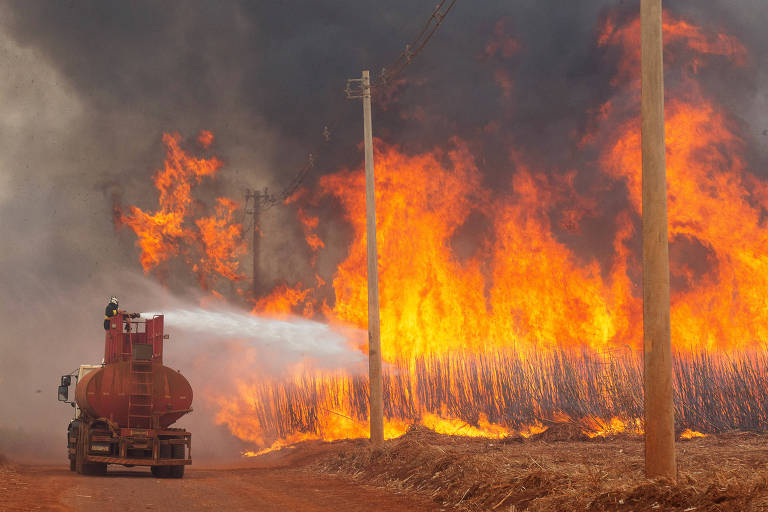
\includegraphics[width=\textwidth]{./image/caminhao_pipa}
	\end{figure}
\end{frame}



\begin{frame}
	\frametitle{Consulta de dados em repositórios online}
	\begin{itemize}
		\item \href{https://visualizador.idesisema.meioambiente.mg.gov.br/}{IDE SISEMA}
		\item \href{https://visualizador.inde.gov.br/}{INDE}
		\item \href{https://datageo.ambiente.sp.gov.br/app/}{DATA GEO}
	\end{itemize}
\end{frame}


\begin{frame}
	\frametitle{Consulta de dados em repositórios online}
	\begin{figure}[H]
		\centering
		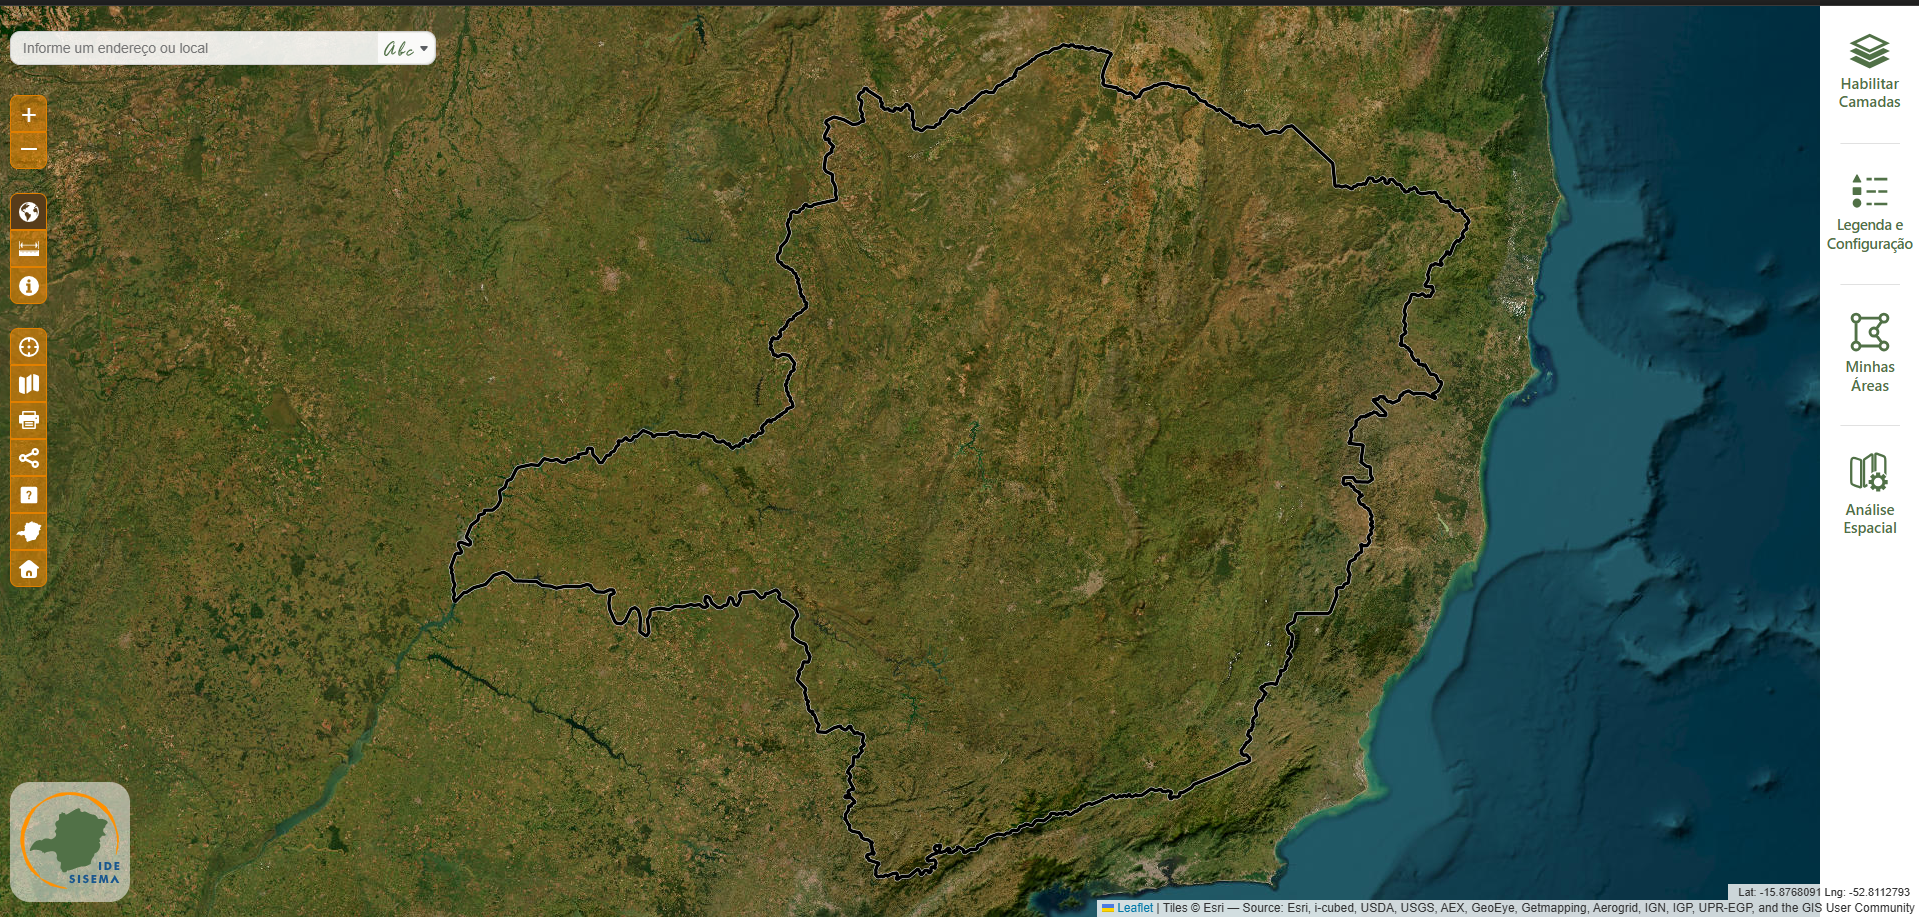
\includegraphics[width=\textwidth]{./image/ide_sisema}
	\end{figure}
\end{frame}

\begin{frame}
	\frametitle{Familiarização com os dados}
	\begin{figure}[H]
		\centering
		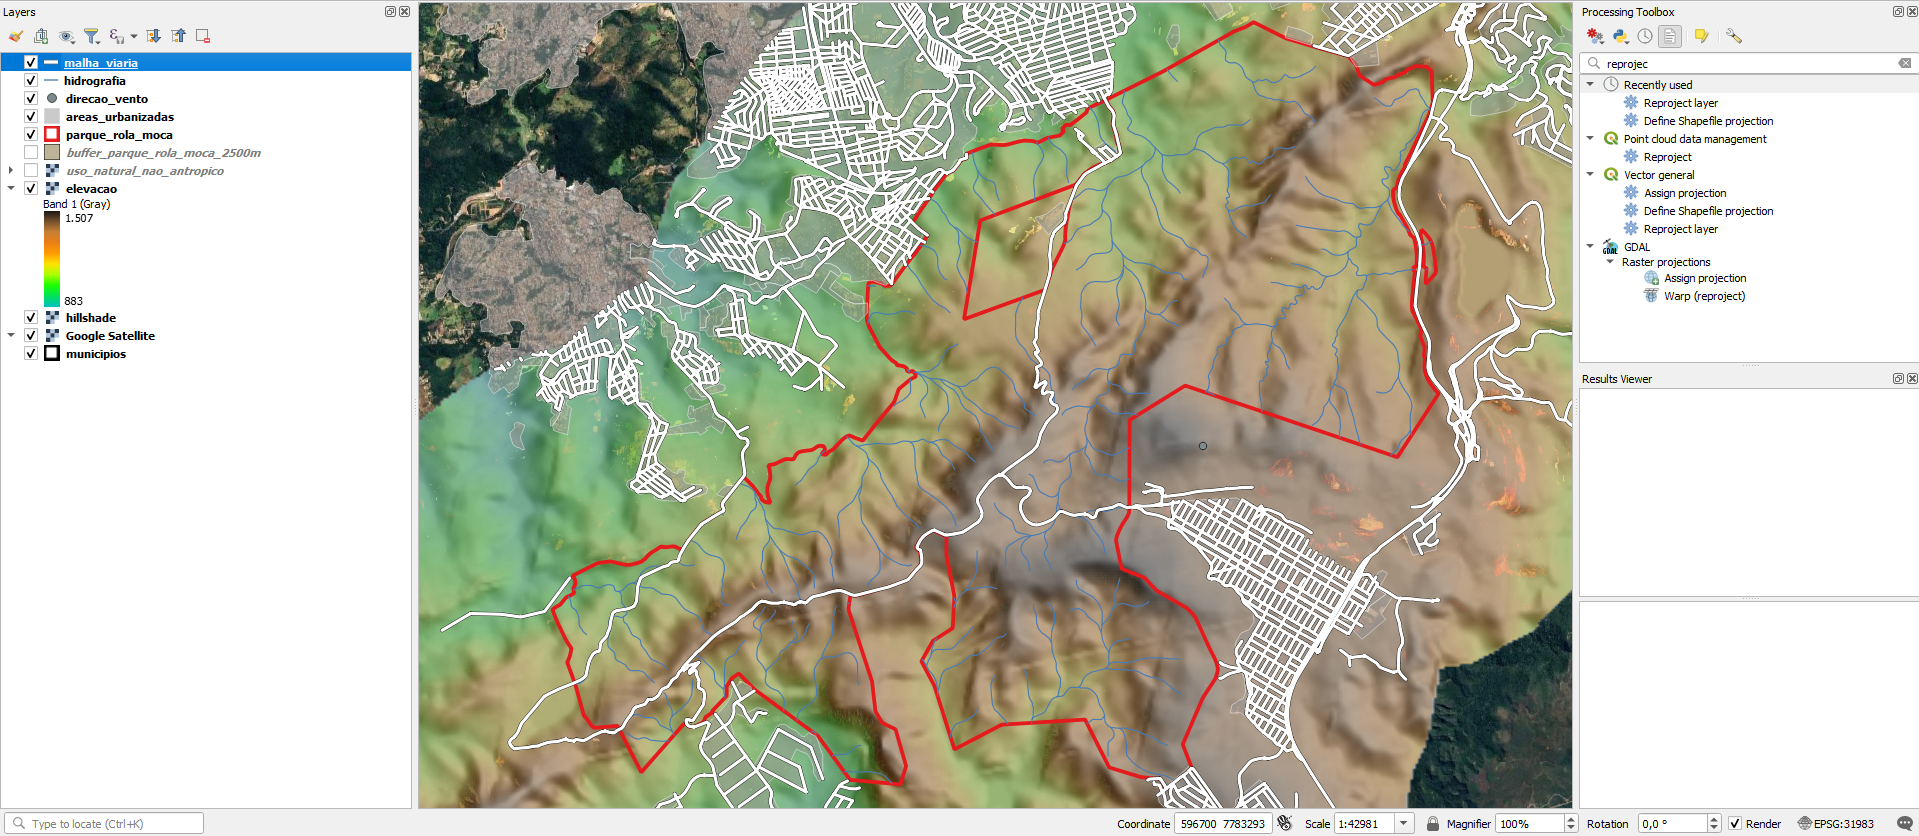
\includegraphics[width=\textwidth]{./image/projeto_qgis}
	\end{figure}
\end{frame}

\begin{frame}
	\frametitle{Familiarização com os dados}
	\begin{itemize}
		\item \textbf{malha\_viaria (estradas e ruas):} \\
		Representa as vias de acesso na região. Servem como caminhos de entrada e saída, tanto para visitantes quanto para veículos de bombeiros em emergências.
		
		\item \textbf{hidrografia (rios e lagoas):} \\
		Mostra os cursos d’água. Essenciais para o abastecimento de água em caso de incêndio.
		
		\item \textbf{direcao\_vento (seta indicando vento):} \\
		Indica para onde o vento sopra. Isso ajuda a prever como o fogo pode se espalhar.
		
		\item \textbf{areas\_urbanizadas (cidades, bairros próximos):} \\
		Representa as áreas já ocupadas por pessoas. Importante proteger moradores e evitar que o fogo chegue perto das casas.
	\end{itemize}
\end{frame}

\begin{frame}
	\frametitle{Familiarização com os dados}
	\begin{itemize}

		\item \textbf{parque\_rola\_moca (limite do parque):} \\
		Área de preservação ambiental que deve ser protegida contra incêndios.
		
		\item \textbf{buffer\_parque\_rola\_moca\_2500m (zona de 2,5 km ao redor do parque):} \\
		Uma faixa de proteção. Mostra áreas próximas ao parque que podem sofrer influência direta de incêndios.
		
		\item \textbf{uso\_natural\_nao\_antropico (áreas de vegetação natural):} \\
		Indica áreas antropizadas e não antropizadas (naturais)
		
		\item \textbf{elevacao (mapa de relevo):} \\
		Indica as altitudes do terreno. Áreas mais altas são boas para instalar postos de observação.
	\end{itemize}
\end{frame}
	
\begin{frame}
	\frametitle{Familiarização com os dados}
	\begin{itemize}
		\item \textbf{hillshade (sombreamento do relevo):} \\
		Uma forma de visualizar montanhas e vales, deixando o relevo mais fácil de interpretar no mapa.
		
		\item \textbf{municipios (limite dos municípios):} \\
		Mostra as divisões administrativas. Importante para saber a quem pertence a área em caso de responsabilidade de combate ao fogo.
		
		\item \textbf{Google Satellite (imagem de satélite):} \\
		Foto real da região, como se fosse vista de cima. Ajuda a reconhecer o que existe no local.
	\end{itemize}
\end{frame}


\begin{frame}
	\frametitle{Familiarização com os dados}
	\begin{figure}[H]
		\centering
		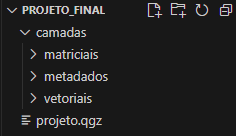
\includegraphics[width=0.8\textwidth]{./image/estrutura_pastas}
	\end{figure}
\end{frame}

\begin{frame}
	\frametitle{Orientações Gerais}
	\begin{itemize}
		\item Todos os arquivos gerados/editados deveram ser mantidos dentro da pasta "projeto\_final";
		\item Deve se manter a organização (dados vetoriais dentro das pastas de arquivos vetoriais, dados matriciais dentro das pastas de arquivos matriciais);
		\item As respostas das perguntas do projeto devem ser respondidas por meio de documento word.
		\item Lembrar de salvar o projeto final do QGIS
	\end{itemize}
\end{frame}

\begin{frame}
	\frametitle{O Projeto}
	Arquivo projeto\_fogo\_gis\.md
\end{frame}





%\bibliographystyle{plain}   % Alterar o estilo da referência caso necessário
%\tiny
\nocite{camara1996geoprocessamento,camara2001introduccao,fitz2008cartografia,silva2003sistemas,thiede2014quantum,tosto2014geotecnologias}
\bibliography{REF}  


\end{document}